\minitoc
In the previous chapter, usage control and distributed ledgers are identified as key technologies for Internet of Things privacy, provided that the distributed ledger can handle requirements in terms of performance. In this chapter, we will introduce the state of the art on \emph{usage control} (Section \ref{S_usage_control}), a privacy-enhancing technology enabling fine-grained dynamic control over the data.

Modern usage control systems now integrate \emph{Information Flow Control} (IFC), a technology that enables the monitoring of the information flow in a system to prevent undue dissemination. The control of information flow, which is compulsory for efficient usage control as it prevents data from escaping the monitoring scope of the usage control system, will be introduced in Section \ref{ss_information_flow_control}. 

Afterward, the state of the art on distributed ledgers will be provided (Section \ref{S_distributed_ledgers}), before focusing on specific IoT aspects. 
Then, distributed ledger privacy (Section \ref{S_privacy_DLT}) and performance (Section \ref{S_DLT_performance}) will be introduced, 
as these two topics are closely related to the Internet of Things concerns.

\rul{A critical analysis of the various technologies and solutions presented is also provided in this chapter, in order to highlight relevant criteria to assess the compatibility with the Internet of Things (Sections} \ref{ss_blockchain_DLT} \rul{and} \ref{ss_performance_consensus_methods} \rul{in particular})
\section{Usage control}
\label{S_usage_control}

In the first chapter, we mentioned usage control as a potential privacy-enhancing technology for the Internet of Things, which could be used jointly with distributed ledgers with the proper integration scheme (\hyperref[obj:23]{\emph{Objective 3}}). In this section, the needed notions of usage control are introduced for a better understanding of this document (Section \ref{ss_ucon_elementaries}), before introducing the system architecture of usage control systems (Section \ref{ss_ucon_architecture}). 
\subsection{Usage control elementaries}
\label{ss_ucon_elementaries}

\paragraph{ABC model.} Usage control is an extension of access control, describing how the data can be used after initial access. It was first proposed by Sandhu and Park as the \emph{UCON} model~\cite{Park2004}. This model extends traditional access control by introducing attribute mutability, as well as new decision factors described by the ABC model (Figure \ref{F_ABC_model}): \emph{Authorizations, oBligations, Conditions}.
In addition, the ABC model considers \emph{subjects and objects}, classic components of traditional access control, and their attributes i.e., \emph{subject attributes} and \emph{objects attributes}. 
\emph{Subject} and \emph{object} are notions taken from access control, such that a \emph{right} enables a subject to access an object in a particular mode e.g., read, write. Note that in usage control, the right does not exist as such, but is determined when the access is initiated by the subject and considering other ABC components. \emph{Usage decision functions} are designed 
to make the determination of a right's existence based on subject and object attributes, authorizations, obligations and conditions.
\emph{Subject} and \emph{object attributes} are properties that can be used during the access decision process. Subject identity is an example of useful subject attributes, but is not mandatory
as it would exclude the possibility of anonymous services. Examples of object attributes are security labels and access-control lists. 

One of the most important innovations of UCON is the introduction of \emph{mutable attributes} that are modified as a consequence of access, while \emph{immutable attributes} are changed as a 
result of administrative action. This is a critical differentiator compared to most access control models and is particularly relevant in IoT contexts due to the dynamicity of the network.
\begin{figure}[t]
\centering
 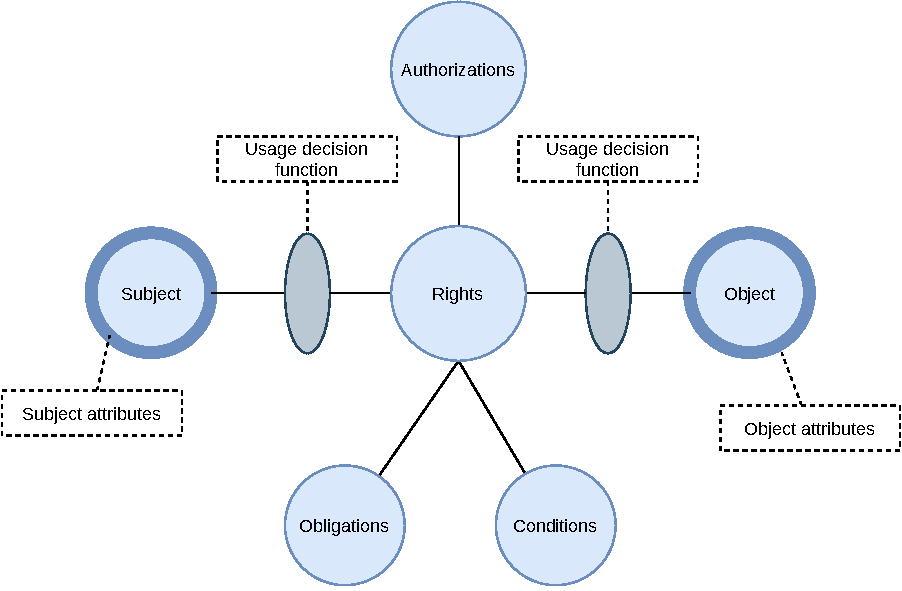
\includegraphics[width=0.8\textwidth]{Images/abc_model.pdf}
\caption{ABC model as defined by Sandhu and Park \cite{Park2004}}
\label{F_ABC_model}
\end{figure} 

 \emph{Obligations} are requirements to be fulfilled by the subject to be granted access. \emph{Conditions} are subject-independent environmental requirements for allowing access. Since attributes are mutable, \cul{authorizations can be checked and obligations fulfilled before or during the access}. They are referred to as pre-authorizations and ongoing-authorizations, or respectively pre-obligations and on-going obligations.
Improving user control over the data is crucial to achieving privacy in IoT systems~\cite{Cha2019}, and usage control provides the technical basis to do so.

\paragraph{Related technologies.} Modern usage control systems rely on information flow control, particularly to prevent data dissemination to uncontrolled areas. Information flow control is extensively discussed in Section \ref{ss_information_flow_control}. Besides, to monitor the use of the data, the usage control system needs to access system calls. This process is intrusive and is a threat to data readers' privacy which must be protected as much as the monitored data. 
To achieve privacy-preserving enforcement of the usage control rules, usage control usually relies on a \emph{Trusted Execution Environment} (TEE)~\cite{Shi2021}. A trusted execution environment is an area on the main processor of a device that is separated from the system's main operating system. It ensures that data is stored, processed and protected in a secure environment. In particular, the data loaded inside a TEE is guaranteed to be protected as regards \emph{integrity} and \emph{confidentiality}. The TEE is installed on the monitored user's machine, to prevent undue processing or dissemination of the monitored data.


\subsection{Usage control architecture}
\label{ss_ucon_architecture}

The components of the usage control system are depicted in Figure \ref{F_ucon_components}. Note that different implementations of a usage control system may not implement every component, or conversely design additional ones. For instance, Martinelli \emph{et al.} \cite{Martinelli2019} introduces components dedicated to the evaluation of obligations called \emph{Policy Obligation Point} to manage distinct kinds of obligations.
\begin{figure}[t]
\centering
 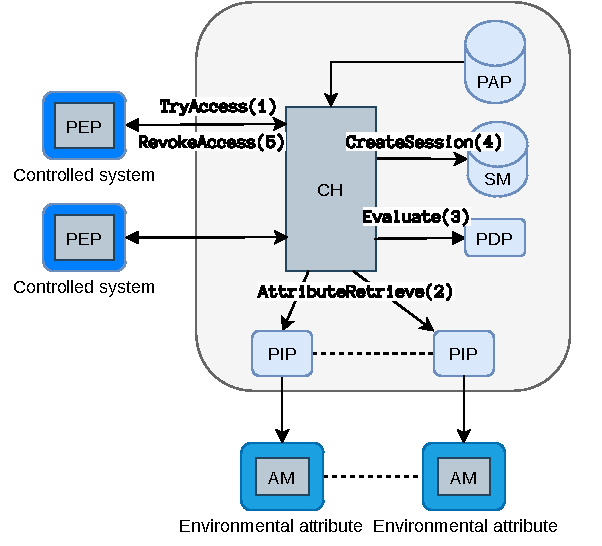
\includegraphics[scale=0.9]{Images/ucon_framework.pdf}
\caption{Usage control architecture, based on~\cite{Rizos2019}}
\label{F_ucon_components}
\end{figure}

The \emph{Usage Control System} (UCS) interacts with \emph{Environmental Attributes} through \emph{Attribute Managers} (AM) to recover the values of the attributes, and with the \emph{Controlled Systems}. 
\begin{itemize}
    \item \emph{PDP}: the Policy Decision Point in charge of the policy evaluation. It takes as input an access request, 
    the corresponding policy and the attributes of both users and context. Then it returns the result of the evaluation: \emph{Permit, Deny, Undetermined};
    \item \emph{PAP}: the Policy Administration Point, which is responsible for creating, modifying, and deleting policies based on the needs of the system and the requirements of the users. It is also the storage point of the policies in the usage control system;
    \item \emph{PEP}: the Policy Enforcement Points are embedded in the Controlled Systems, and intercept access requests and trigger the UCS decision-making process. The PEPs then enforce the policy evaluation result on the Controlled System which requires an access;
    \item \emph{PIP}: the Policy Information Point, an interface so that the UCS can retrieve the values of the attributes from the system environment;
    \item \emph{CH}: the Context Handler, in charge of routing the different processes;
    \item \emph{SM}: the Session Manager stores all active sessions and the information needed for monitoring their status. The SM is composed of an \emph{Access Table} that stores information about the current ongoing sessions to be able to continuously enforce policies. Usually, Access Tables are implemented by a database whose entries refer to a session and contain at least the session identifier, the access request and the session status i.e., pending, active, revoked or ended.
\end{itemize}


\textbf{Workflow.} The workflow between the different components of the usage control system after receiving an access request is shown in Figure \ref{F_ucon_components} and is composed of the following messages \cite{Rizos2019}. When a user requires access, the PEP sends a \texttt{TryAccess} message to the CH. The CH fetches the environmental attributes from the PIP (\texttt{\justify AttributeRetrieve}) and the policy from the PAP, and forwards them to the PDP to evaluate the policy (\texttt{Evaluation}). The PDP decides to accept or reject the request with a
 \emph{PERMIT} or a \emph{DENY} message, then sends the decision to the CH which forwards it to the PEP. If the answer is \emph{PERMIT}, a unique SessionId is assigned to the access request (\texttt{createSession}) and the Session Manager (SM) is updated. The PEP then sends a \texttt{startAccess} message to the CH, to signal the start of the access. If the UCS detects a policy violation during the continuous monitoring, the CH informs both the PEP and the SM that the session is terminated by sending the \texttt{revokeAccess} message. It is also possible that the user asks to end the session itself, by sending the \texttt{endAccess} message. The CH tells the SM to delete the session details, and the PIP to unsubscribe the attributes related to this session.

\subsection{Information flow control}
\label{ss_information_flow_control}

We introduced usage control as a dynamic and flexible access control technology. It enables data owners to enforce policies for their data, 
by defining authorizations, but also obligations, which are actions to be performed before, during or after being granted access, and conditions bearing on the system and environment attributes, e.g., the time.

 Several methods exist to limit information disclosure, including usage control but also access control lists, firewalls or cryptography. However, although these methods do impose limits on the information that is released by a system, they do not provide any guarantees about information \emph{propagation}. 
 Monitoring data dissemination is valuable in information security to prevent leaks, but also for usage control as information could be disseminated outside the scope of the usage control system. 
 \emph{Information Flow Control} (IFC) is a mechanism introduced to enforce information flow policies in a system. Several methods to implement information flow control have been proposed in the literature:
 \begin{itemize}
    \item Run-time mechanisms that tag data with \emph{information flow labels} have been employed at the operating system level and the programming language level \cite{Hu2021};
    \item \emph{Static program analyses} have also been developed to ensure information flows within programs conform with policies \cite{Zheng2007};
 \end{itemize} 

 \textbf{Taxonomy.} Information flow control techniques can be characterized and compared using the following features \cite{Denning1976, Hu2021}. 
\begin{enumerate}
    \item \emph{Operator precision}: How are security classes updated? 
    \begin{itemize}
        \item Conservative: IFC uses a least upper bound;
        \item Precise: IFC considers the value of the data;
        \item Hybrid: IFC performs a tradeoff between accuracy and computational cost.
    \end{itemize}
    \item \emph{Security properties}: Which security properties are guaranteed?
    \begin{itemize}
        \item Confidentiality: IFC prevents leakage of sensitive information;
        \item Integrity: IFC prevents undue modification of data;
        \item Isolation: IFC forbids communication between two agents with different trust levels;
        \item Constant time: IFC captures information flows through runtime variations;
        \item Design integrity: IFC technique detects malicious information flows triggered by design modifications;
    \end{itemize}
    \item \emph{Level of Abstraction}: What is the level of abstraction of the information flow model?
    \begin{itemize}
        \item System: IFC considers flows at the system level;
        \item Algorithmic: IFC is deployed during high-level synthesis (HLS). 
        HLS involves transforming an abstract, algorithmic-level description into a lower-level, hardware-specific implementation that can be synthesized into digital circuits;
        \item Architecture: IFC is deployed at the Instruction Set Architecture (ISA) level. 
        The Instruction Set Architecture is the interface between a computer's software and hardware components, defining the set of instructions that a processor can execute and the memory model it operates on;
        \item RTL: IFC targets register transfer level (RTL);
        \item Gate: IFC occurs at the gate level. A gate-level netlist is a representation of a digital circuit at the lowest level of abstraction;
        \item Circuit: IFC targets analog and mixed-signal hardware designs.
    \end{itemize}
    \item \emph{Verification Technique}: Which verification techniques are supported?
    \begin{itemize}
        \item Simulation: IFC determines information flows using simulation tools;
        \item Formal: IFC checks security properties using formal methods, e.g., theorem proving, equivalence checking...;
        \item Emulation: IFC relies on hardware emulation of information flow behaviors;
        \item Virtual prototyping: IFC creates a software version of the hardware to monitor information flow;
        \item Runtime: Dynamic IFC during runtime.
    \end{itemize}
\end{enumerate}

\subsection{Conclusion on usage control}

\sul{As a conclusion, we summarize the key elements of usage control needed for the rest of this document. First, usage control is an extension of access control introducing attribute mutability, obligations and conditions. These concepts are useful to handle IoT aspects, in particular the dynamicity of the network, and to design fine-grained policies that consider the users' actions and the system's state, during the whole access phase (including before and after the access).
The usage control system (UCS) is responsible for enforcing usage control, and its components are partly located on the end devices under the form of policy enforcement points. Finally, modern usage control systems are complemented by information flow control, to monitor the data dissemination and prevent malicious users from sending the data outside of the UCS scope.} 
\section{Distributed ledgers}
\label{S_distributed_ledgers}
Distributed ledgers, particularly blockchains, have been actively studied as a promising technology for the Internet of Things privacy \cite{Rifi2017, Zhaofeng2021, Goyat2022, Rajasekaran2023, Bao2023} notably for access control, auditing and data storage \cite{Cha2019}. 
As a potentially relevant solution to \hyperref[obj:1]{\emph{Objective 1}}, the focus will be given in this section to distributed ledger technologies and why they can be useful for the Internet of Things.

General principles of distributed ledger technologies (Section \ref{ss_DLT_elementaries}) and common consensus methods (Section \ref{ss_consensus_methods}) will first be introduced in this section, before distinguishing distributed ledgers from blockchains (Section \ref{ss_blockchain_DLT}).

 Privacy issues in distributed ledgers and current means to mitigate them are discussed in Section \ref{S_privacy_DLT}. Distributed ledger performance is finally considered in Section \ref{S_DLT_performance} along with the relevant metrics to measure it.
% The following Section \ref{S_DLT_IoT} introduces the specific features and constraints of distributed ledgers when used in the Internet of Things context. 
\subsection{Blockchain elementaries}
\label{ss_DLT_elementaries}

\textbf{History.}
In 1996 the NSA published a report "How to make a mint: the cryptography
of anonymous electronic cash" \cite{Law1997}, to express its concerns about
electronic currencies. This document raises several potential problems, which
are still relevant today:
\begin{enumerate}
\item The problem of \emph{double spending}. In the case of offline payments, it is not possible to guarantee that a coin will only be spent once;
\item To transfer money, the user must use an electronic \emph{wallet}, developed by a company. This can be seen as a
trusted third party that can potentially act against the will of its owner, e.g., by tracing the transactions. The latter can also be in charge of checking that there is no double spending;
\item All the security of the protocol lies in the chosen \emph{cryptographic functions}, which may be insecure.
\end{enumerate}

In 1997, Adam Back proposed a \emph{proof-of-work} method, under the name
Hashcash \cite{Back2002}. The principle is to perform a given amount of work, requiring CPU resources, to access a service. If a user is legitimate, this work is negligible, while in the case of a malicious person
accessing the service repeatedly, this amount of work becomes considerable. This technique is used for example to fight against \emph{spam} or \emph{denial of service}.

In 2008, Satoshi Nakamoto wrote the founding paper for Bitcoin \cite{Nakamoto2008}. This name appears to be a pseudonym, and the real identity of this person, or group of people, remains a mystery to this day. This article describes the structure and operation of the Bitcoin protocol. The implementation of Bitcoin came the following year, in 2009, under the name
Bitcoin-QT. This is also the first time the word \emph{blockchain} is used.

Five years later, in 2013, Vitalik Buterin introduces Ethereum \cite{Buterin2014}, a novel blockchain network with the possibility to execute \emph{decentralized applications} (DApps) \emph{via} smart contracts. \emph{Smart contracts} are "computerized transaction protocol that executes the terms of a contract" \cite{Szabo1994}, enabling decentralized execution of code with predetermined conditions, without the intervention of a third party.

\textbf{Blockchain architecture.} Blockchains are usually decoupled in several layers, depending on the model, to fully describe the underlying architecture of a blockchain. While the models can differ, the most common model is composed of six layers \cite{Wen2021, Issa2023}, discussed next and shown in Figure \ref{F_layers}. 

\begin{figure*}[t]
\centering
 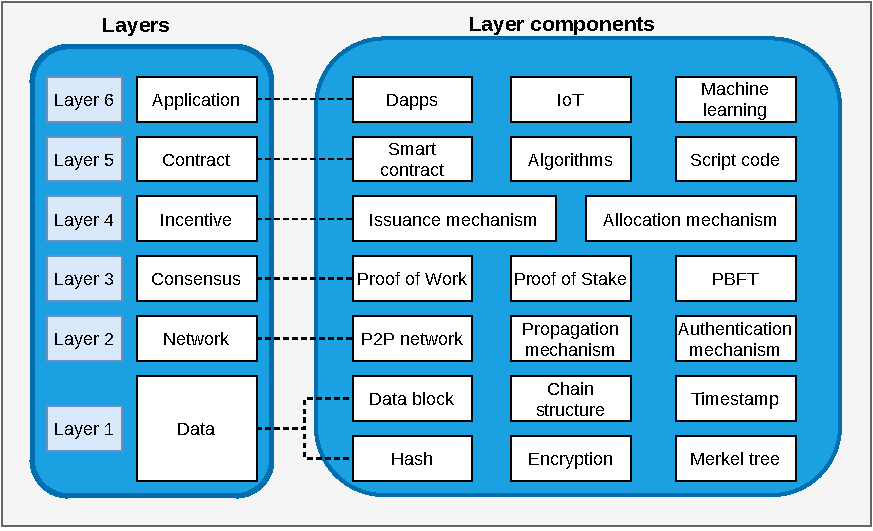
\includegraphics[width=\textwidth]{Images/layers.pdf}
\caption{Blockchain architecture in six layers, based on \cite{Yuan2018}} 
\label{F_layers}
\end{figure*}

The first \emph{data layer} involves the techniques required for storing transaction records. Each block in the ledger stores a set of verified, timestamped and hashed transactions, in the form of a Merkle tree \cite{Yuan2018, Issa2023}.

The \emph{network layer} (layer 2) includes the network aspects, such as the communication and verification mechanisms, including authentication. Nodes in a blockchain network usually interact forming a peer-to-peer (P2P) decentralized network. The network layer helps in broadcasting, forwarding and verifying transactions.  When a node creates a transaction, it signs it with its private key then broadcasts it to its neighbors. The neighbors verify this transaction with its public key. If the transaction is valid, it is added to the blockchain and broadcast to the other nodes of the network, or discarded otherwise \cite{Yuan2018, Issa2023}.

The \emph{consensus layer} (layer 3) is used by the network of nodes to reach an agreement on the state of the blockchain. The blockchain state includes the valid transactions, the blocks in the ledger and their order, as well as the next block to be added. Numerous consensus algorithms have been designed for blockchains, which are extensively discussed in Section \ref{ss_consensus_methods}.

The \emph{incentive layer} (layer 4) is a fundamental part of the blockchain architecture that encourages users to contribute to the network, usually with economic incentives.
The incentives are given to specific nodes so that they verify the blocks and keep the decentralized nature of the blockchain network. 

The \emph{contract layer} (layer 5) includes smart contracts, but also algorithms and script codes to extend the logic of transactions. This layer enables to devise more complex business rules, automatically performed when predetermined conditions are fulfilled.

The \emph{application layer} (layer 6) includes a wide range of applications that leverage blockchain properties. It can include generic applications, such as machine learning or the Internet of Things. Decentralized applications (DApps) are encompassed in this layer as well.

\begin{figure*}[t]
\centering
 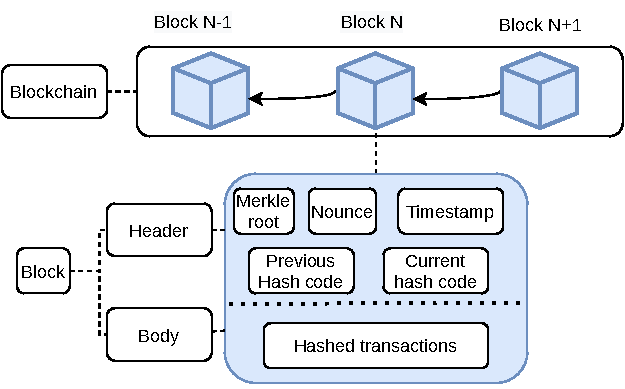
\includegraphics[width=0.7\textwidth]{Images/blockstruct.pdf}
\caption{Block composition - based on \cite{Issa2023}} 
\label{F_blockstruct}
\end{figure*}

\begin{samepage}
\textbf{Block composition.} \sul{The blocks composing the transaction ledger are composed of a header and a body, shown in Figure} \ref{F_blockstruct}. \sul{The body part of the block holds hashed transactions, while the header is constituted of these parts} \cite{Nakamoto2008, Issa2023}:

\begin{enumerate}

    \item \sul{\emph{Merkle Root}: The Merkle root is a hash value computed from the set of all transactions included in the block. It is used to cryptographically prove that all transactions within the block are valid and unchanged} \cite{Merkle87}.
    
    \item \sul{Nonce: a nonce is an arbitrary number that can be used just once in a cryptographic communication. Nonces are used in proof-of-work systems to vary the input to a cryptographic hash function to obtain a hash for a certain input that fulfills certain arbitrary conditions, notably on difficulty;} 
    
    \item \sul{Previous Hash Code: This field contains the hash value of the previous block in the blockchain. It forms the link between blocks and ensures the integrity and chronological order of the blockchain.}
    
    \item \sul{Timestamp: The timestamp indicates the exact time when the block was created. It provides a reference point for ordering blocks and contributes to the overall consensus mechanism of the blockchain.}
\end{enumerate}
    
\end{samepage}

\subsection{Consensus methods}
\label{ss_consensus_methods}

Consensus methods (layer 3, as introduced in Section \ref{S_distributed_ledgers}) are very diverse and have different advantages and drawbacks regarding performance, security and privacy. Due to their significant impact on the network characteristics, the most popular consensus mechanisms are discussed next.

\textbf{Proof of Work.}
The proof of work (PoW) is a consensus method based on a computation race. The first participant who solves the computation puzzle wins the right to add the next block to the transaction ledger.
 It was popularized by the Bitcoin blockchain as the first consensus method for blockchains \cite{Nakamoto2008}.
The user appending the new block to the ledger is called the \emph{miner}. The computation puzzle is most commonly based on a hash function, where the users have to find a nonce to solve the given problem.
 It consumes a lot of computational resources, raising environmental concerns \cite{Stoll2019, Sharma2023}.

Blockchain networks based on proof of work are vulnerable to the 51\% attack, which is a potential security vulnerability in blockchain networks where a single entity or group of entities gains control 
of more than 50\% of the network's mining power \cite{Aponte2021}. 
If an attacker gathers the majority of the mining power, it allows him to spend its funds multiple times, reorganize the blockchain by creating a longer chain with alternative transactions, or block the incoming transactions.

\textbf{Proof of Stake.} The proof of stake (PoS) was proposed to overcome the issues of the proof of work, in particular the high energy and computational resource consumption. In contrast with the proof of work, the PoS does not rely on a computation race but rather on an economic stake as proof to select the next validator.
The first cryptocurrency to use proof of stake is Peercoin (PPCoin)\cite{King2012}.
Ethereum, Bitcoin's main competitor, has replaced proof of work with proof of stake in its current version Ethereum 2.0. 
While proof of stake is not threatened by the 51\% attack\footnote{Yet, if a single entity or a group were to control the majority of the stake, they would have disproportionate influence over the network's consensus and decision-making process}, it is endangered by the \emph{Nothing at Stake} problem. 

The \emph{Nothing at Stake} problem arises when validators in a PoS network
 are not financially incentivized to follow the rules and behave honestly. Since validators do not have to spend computational resources or energy to create blocks in PoS, there is no direct cost associated with attempting to create multiple competing blockchains.
 This creates a scenario where validators can potentially create multiple valid chains in an attempt to double-spend or disrupt the network without any economic consequences. 
However, the \emph{Nothing at Stake} problem is not a practical vulnerability in most PoS protocols. This is because PoS protocols usually have mechanisms implemented to prevent or mitigate this problem. 
For example, penalties or slashing mechanisms can be used to punish validators who attempt to create multiple competing chains.

There are several variations of the proof of stake that are designed to adjust PoS performance metrics to fit specific use cases.
The \textbf{Delegated Proof of Stake} (DPoS) is a version of PoS where stakeholders vote to elect a set of delegates or validators who are responsible for producing blocks and maintaining the blockchain. These elected validators take turns creating blocks on behalf of the stakeholders who elected them.
The \textbf{Leased Proof of Stake} (LPoS) allows users to lease their stake or balance to a chosen delegate, who then includes their stake in their own validator's pool. This allows users with smaller stakes to participate in the block production \cite{Salimitari2020}.
The \textbf{Liquid Proof of Stake} (also LPoS) introduces a concept of liquidity, where stakeholders can freely transfer or trade their staked tokens while still participating in the consensus mechanism. This allows for more flexibility and liquidity compared to traditional staking mode \cite{Breitman2014}.

The \textbf{Proof of Authority} (PoA) is a variant of the proof of stake where the \emph{identities} and the \emph{reputation} of the nodes \emph{are at stake} rather than a cryptocurrency asset. The time to reach the consensus and the latency is better compared to the proof of work, but not as good as the actual proof of stake~\cite{Raghav2020}.
One significant contribution to its popularity was the introduction of the PoA consensus algorithm by Gavin Wood, the co-founder of Ethereum, in the Ethereum network's \emph{Parity} client \cite{Ekparinya2020}.
In the following, only the conventional PoS, the delegated and the proof of authority are considered, as both liquid and leased proofs do 
not have an impact on network metrics, but have an economic rationale.

\textbf{Proof of Elapsed Time.} In the Proof of Elapsed Time (PoET), the miner is chosen at random based on a timer. The user whose timer expires first becomes the miner. This consensus method has several benefits,
including a higher throughput and a low latency.
However, its main drawback is its reliance on Intel's SGX, as the correctness of the timer execution must be verified within a \emph{trusted execution environment}, implying PoET's governance is centralized.
 
The Proof of Elapsed Time consensus mechanism was popularized through its implementation in the Hyperledger Sawtooth blockchain platform, developed by the Linux Foundation. 
Intel, the company behind the creation of PoET, actively contributed to its promotion and adoption by highlighting its energy efficiency and scalability benefits compared to traditional consensus mechanisms like Proof of Work (PoW) \cite{NDSSWang2022}.

\textbf{Practical Byzantine Fault Tolerance.}
The Practical Byzantine Proof Tolerance (PBFT) is a voting-based consensus method. All the nodes are involved in the voting process and the consensus is reached when more than two-thirds of the nodes agree 
upon the next block. As a consequence, the network can handle malicious behavior from at most a third of the nodes, 
which is low compared to the 51\% assumption in the proof of work networks~\cite{Aponte2021}. PBFT is consequently efficient in private blockchains, but not for public blockchains which
have a lower tolerance to malicious nodes~\cite{Salimitari2020}. In addition, the voting process does not scale well, as PBFT generates a significant network 
overhead \cite{Salimitari2020}. 
Practical Byzantine Fault Tolerance (PBFT) was introduced by Miguel Castro and Barbara Liskov \cite{Castro1999}.
 The paper introduced the PBFT algorithm as a solution for achieving consensus in distributed systems under the presence of Byzantine faults.

A delegated version of the practical byzantine fault tolerance is used as well in cryptocurrencies called \emph{dPBFT}. dPBFT stands for \emph{Delegated Proof of Byzantine Fault Tolerance}. It is a consensus algorithm that builds upon the original PBFT algorithm. dPBFT was introduced to improve the scalability and performance of PBFT by allowing a smaller subset of nodes, known as \emph{delegates} or \emph{representatives}, to handle the consensus process on behalf of the entire network. This delegation reduces the communication and computational overhead compared to traditional PBFT, making it more suitable for large-scale distributed systems.
 dPBFT and the concept behind it have been popularized by the NEO cryptocurrency project, which implemented the dPBFT consensus algorithm as its underlying consensus mechanism \cite{Zhan2021}. 
\subsection{From blockchains to distributed ledgers}
\label{ss_blockchain_DLT}
 
 While blockchains are the most well-known instances of distributed ledgers for cryptocurrencies, the notion of \emph{Distributed Ledger Technology} (DLT) is broader and includes several other technologies of interest that are introduced in this section. 
 
 First, a distributed ledger can be completely disconnected from the notion of cryptocurrency, e.g., distributed databases. Besides, some cryptocurrencies do not build their transaction ledger using blockchains, but rather using different mathematical structures. The most used alternatives to blockchain in cryptocurrencies are the \emph{directed acyclic graphs} (DAGs) and the \emph{hashgraphs}.

  \begin{figure}
    \centering
    \begin{subfigure}[b]{0.48\textwidth}
        \centering
        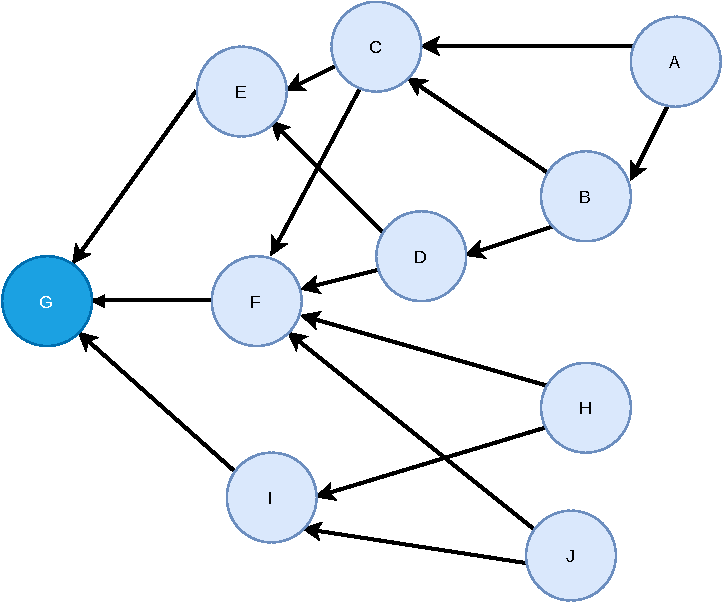
\includegraphics[width=0.8\textwidth]{Images/DAG.pdf}
        \caption{Directed acyclic graph (DAG). Transaction $A$ directly approves $B$ and $C$, indirectly approves $E$, $F$ and $G$. $G$ is the original transaction,
        approved by all other transactions \cite{Popov2017}.}
        \label{F_DAG}
    \end{subfigure}
    \hfill
    \begin{subfigure}[b]{0.38\textwidth}
        \centering
        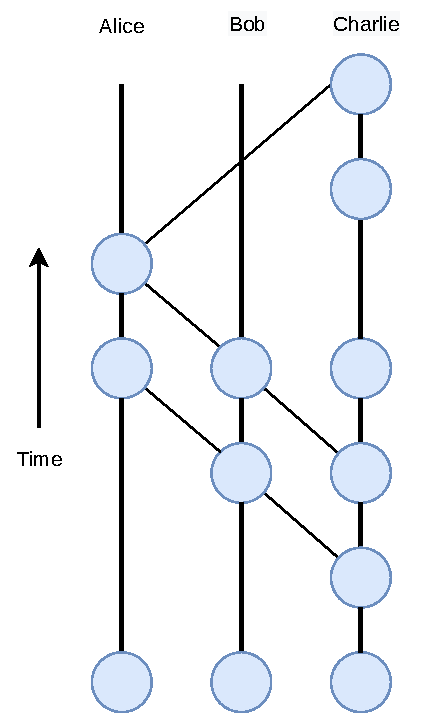
\includegraphics[width=0.63\textwidth]{Images/hashgraph.pdf}
        \caption{Hashgraph, representing the gossip history. If Alice receives gossip from Bob,
         the event is marked by a vertice in the Alice column, with two edges going downward
        to the preceding gossip events by Alice and Bob \cite{Baird2018}.}
        \label{F_hashgraph}
    \end{subfigure}
    \hfill

       \caption{Alternatives to blockchains to build transaction graphs.}
       \label{F_alternative_DLT}
\end{figure} 


 \textbf{Directed acyclic graph.} Unlike a traditional blockchain, where transactions are organized in linear blocks, a directed acyclic graph allows multiple transactions to be confirmed concurrently, 
 enabling greater scalability and potentially faster transaction processing times. Several cryptocurrencies rely on directed acyclic graphs to build the transaction ledger
 such as IOTA \cite{Popov2017}, Obyte~\cite{Churyumov2017} and Nano~\cite{LeMahieu2017}. IOTA is by far the most studied DAG-based distributed 
 ledger in the scientific literature \cite{Conti2022, Carelli2022, Guo2023, Naresh2023}.
 Though DAG-based technologies slightly differ, they share several interesting properties:
 \begin{itemize}
    \item small transactions fees, or even no transaction fees at all;
    \item writing transaction is not energy-intensive;
    \item throughput is high after the bootstrapping stage and increases with the number of users;
    \item users add their transactions directly to the network without relying on any intermediaries, such 
    as miners or gateways.
 \end{itemize}

In general, a DAG-based distributed network builds its transaction ledger as detailed next. The transactions
issued by nodes constitute the vertices of the transaction graph. There is only one transaction by vertice, in 
contrast with blockchains that usually store multiple transactions in one block. The edges of the graph are obtained as follows:
when a new transaction arrives, it must approve two previous transactions. These
approvals are represented by directed edges, as shown in Figure \ref{F_DAG}. If there are no
directed edges between two transactions $A$ and $B$, but there is a directed
path of length at least two from $A$ to $B$, we say that $A$ indirectly approves $B$.
There is an original transaction, which is approved directly or indirectly by all the transactions.
 
 \textbf{Hashgraph.} Hashgraph is a distributed ledger technology designed as an alternative to blockchains.
  The hashgraph technology is currently patented and used by the public ledger Hedera \cite{Baird2018}. Hashgraphs
  have been studied in the literature as possible alternatives to blockchains, in particular in the context 
  of the Internet of Things \cite{Bansal2020, Gao2022, Jha2022, Tarlan2022}. The claimed features of Hedera's hashgraph are the following:
  \begin{itemize}
    \item very high transaction throughput and low latency;
    \item \emph{fairness} in the ordering of transactions by using a consensus algorithm that considers the timestamp of each event.
     This approach aims to prevent unfair advantages or biases among participants, in particular in use cases involving real-time pricing such as stock markets;
     \item resilience against denial of service attacks thanks to asynchronous byzantine fault tolerance (aBFT) consensus. aBFT is 
     a version of PBFT for asynchronous networks; 
  \end{itemize} 

While these claims are attractive, Hedera's hashgraph lacks evaluation and peer review for the scientific community. 
In particular, the claim regarding throughput, up to 500.000 transactions per second \cite{Baird2018}, is way above the current
standards (24.000 TPS for Visa). Hedera claims that the network throughput is only limited by bandwidth, which requires each network 
node to be able to download and upload the transactions, which set high requirements on network nodes. Besides, the 
claims should be verified based on empirical evidence, performance benchmarks, and independent research.

\textbf{Hashgraph consensus protocol.} The core of the hashgraph consensus is called \emph{gossiping}. The gossip protocol unfolds as follows. 
The first member (Alice) chooses another member at random (Bob), and then Alice tells Bob all of the information she has about the current status 
of the ledger. Alice then repeats with a different
random member. Bob repeatedly does the same, as well as all other members of the 
network. Consequently, if a single member becomes aware of a new transaction, 
the information is spread exponentially fast through the community until every member is aware of
it.

In hashgraph, the participants do not only gossip transactions, but also the hashgraph itself, 
a process which is referred to as \emph{gossip about gossip}.
Gossiping a hashgraph gives the participants a great deal of information. 
If a new transaction is placed in the payload of an event, it will quickly spread to all
members, until every member knows it. A participant can learn about new transactions, know 
when exactly a participant learned about a given transaction, and also know
exactly when a participant learned the fact that another participant had learned of that transaction by transitivity.

The gossip history is therefore represented as a directed graph. The history of any
gossip protocol can be represented by a graph where each member
is a line composed of vertices. When Alice receives gossip from Bob,
telling her everything he knows, that gossip event is represented
by a vertex in Alice's line, with two edges going downward
to the immediately-preceding gossip events by Alice and Bob. 
The hashgraph is represented in Figure \ref{F_hashgraph}.

\subsection{Conclusion on distributed ledgers}

\sul{Distributed ledgers, whose most famous instances are blockchains, are in fact more diverse and encompass distributed databases as well as ledgers built using hashgraphs or directed acyclic graphs. Apart from the structure of the transaction graph, the main distinctive feature of distributed ledger is the consensus method, used to decide who can write the transactions and how. The consensus method has a strong impact on the network's security and performance, which we will discuss in Section} \ref{S_DLT_performance}. \sul{Besides, distributed ledgers are confronted to privacy challenges that are discussed in the next Section} \ref{S_privacy_DLT}

\section{Preserving privacy in distributed ledgers}
 \label{S_privacy_DLT}

While distributed ledger transactions are thought to be anonymous, the reality is more balanced. Public blockchains do not require identifying information to make a
transaction.  Yet, access to transactions and their content is not restricted. The transactions disclose information about the different parties involved and create risks of inference. Interested third parties also automatically collect and analyze
this information, for several purposes including law enforcement \cite{Harrigan2016}. By default, public blockchains only provide pseudonymity, or anonymity provided
the linkage between the pseudonym and the real identity is not possible. However, 
several behaviors drastically make re-identification easier, which are discussed in the section \ref{ss_de_anonymisation}.
In the next section, we detail the privacy threats for distributed ledger technology, based on LINDDUN privacy threat modeling \cite{Wuyts2015}.

\subsection{Privacy threat modeling.}
\label{ss_privacy_threat_modeling}
LINDDUN is a privacy threat modeling framework \cite{Wuyts2015} to reason about potential privacy concerns in 
a systematic and structured way. It is structured according to seven threat types captured in the 
acronym LINDDUN. LINDDUN is used in this section to identify the main privacy threats in distributed ledgers 
so that the risks addressed by the privacy-preserving tools detailed in the following (Section \ref{ss_obfuscation_coin_mixing_merge_avoidance})
are clearly expressed.

\textbf{Linking.} Linking is the association of data items or user actions to learn more about an 
individual or a group. In blockchains, linking threats can be done by linking several transactions 
together to deduce the consumption habits of a user, or by linking senders and receivers of transactions.

\textbf{Identifying.} The identifying threat is the risk of learning the identity of an individual, even though 
it wants to remain anonymous. In distributed ledger technologies, the main risk is breaking the pseudonym, i.e., the 
address of a user in the blockchain, to disclose its true identity. This is usually achievable 
by combining blockchain data with external information, such as network data, by identifying 
from which IP address a transaction originates.

\textbf{Non repudiation.} The non-repudiation threat is the ability to attribute a claim to an individual, e.g., read a message. 
The system maintains evidence regarding some actions of facts, which implies deniability claims, like log files or metadata. 
Non-repudiation is a counter-intuitive notion when it comes to privacy threat assessment, as 
in \emph{security threat modeling} such as STRIDE \cite{Howard2006}, repudiation is conversely 
considered as the security risk. In security, it is more relevant to prevent a malicious user 
from denying it performed a forbidden action, while for privacy preservation, it is better 
to be unable to attribute actions to individuals. An example of non-repudiation risk 
for a blockchain user is the impossibility to deny it performed a transaction.

\textbf{Detecting.} Detecting is the ability to deduce the involvement of an individual through observation. 
Notably, as the ledger is public, it is possible to see if a user made transactions in a blockchain 
network as its address is recorded in the transaction. It is an issue when combined 
with identification attacks, or if the motive of the transaction can be disclosed.

\textbf{Data disclosure.} Data disclosure is the excessive collection, storage, processing or sharing of personal data.
This is not a general threat in blockchains and distributed ledger technologies and is rather implementation-dependent.

\textbf{Unawareness.} Unawareness corresponds to insufficient information and involvement of individuals in the 
processing of their personal data. It is also not a general risk.

\textbf{Non-compliance.} The last non-compliance threat reflects the deviation from security and data management best practices, 
standards, and legislation. Distributed ledger technologies can be legal conundrums regarding
 the EU General Data Protection Regulation (GDPR) \cite{EUdataregulations2018, Haque2021}:
\begin{enumerate}
    \item Article 3 - \emph{Territorial scope}. Article 3 is about
    controlling the user data from being processed and stored outside 
    the geographical area of the EU. In the case of the public blockchain, it is difficult since
    the nodes are distributed worldwide. Private blockchains can conversely have nodes 
    that are located in the same region;
    \item Article 16 and 17 - \emph{Right to deletion and modification}. 
    One of the most important legal issues for blockchains 
    is Article 17 of GDPR,
    about the \emph{right to be forgotten}. That means the concerned
    organizations should delete the user data if the users request it. 
    Since information inside the blockchain cannot be
    removed, it directly contradicts Article 17.
    This is also true for Article 16 \emph{right to rectification} as data cannot be edited either.
    \item Article 4 states the definition of \emph{personal data}, data \emph{controller},
    and data \emph{processors}. Articles 24 and
    28 describe data controllers’ and processors’ purposes and
    responsibilities. Identifying data controllers and processors is hard for blockchains since no centralized authority is
    controlling the nodes or is accountable for them.
\end{enumerate}



\subsection{Breaking pseudonymity in blockchains}
\label{ss_de_anonymisation}

Most public blockchains including the two most popular, Bitcoin and Ethereum, only provide pseudonymity under the form of an address. Anonymity would be provided if it is not possible to link the pseudonym and the real identity. However, several behaviors of users and techniques significantly ease the re-identification process.

\textbf{Clustering.} Address clustering in the context of blockchain refers to the process of identifying multiple addresses that belong to the same user or entity by analyzing their transactional behavior on the blockchain \cite{Huang2017}. It is a method used to de-anonymize blockchain transactions and can potentially reveal the identity of the user or entity behind the transactions. Address clustering is a common technique used by law enforcement \cite{Harrigan2016} agencies to investigate illicit activities such as money laundering and terrorist financing.

\textbf{Address reuse.} Address reuse in blockchains occurs when the same public address is used for multiple transactions. This can be problematic for several reasons. First, for privacy, when a user reuses an address for multiple transactions, it becomes easier for anyone to track the user's transactions as it requires to link one address to an identity. Conversely, using a different address for each transaction requires repeating the process of re-identification several times, which is time-consuming. Additionally, address reuse is a problem for security, as the leak of only one private key enables a malicious agent to steal all the funds of a user.

\textbf{Network analysis.}  By monitoring network traffic and analyzing the timing, size and value of transactions, it is possible to infer relationships between addresses and potentially identify the real-world identities hidden behind the 
pseudonym address. For instance, heuristics have been developed to identify ownership relationships between Bitcoin addresses and IP addresses \cite{Koshy2014},
significantly facilitating re-identification.

\subsection{Obfuscation using coin mixing and merge avoidance}
\label{ss_obfuscation_coin_mixing_merge_avoidance}
Coin mixing services allow users to mix cryptocurrency coins
to enable unlinkable payments and prevent tracking of honest users’ coins by both the service provider i.e. the \emph{coin mixer} or \emph{coin tumbler}, and the users themselves.
The easy bootstrapping of new users and backward
compatibility with cryptocurrencies are attractive features of this service, which
has recently drawn the attention of both academia and
industry. While useful for privacy preservation, coin mixers face several technical challenges such as decentralization to be able to meet their requirements as regards privacy.

\textbf{Principles of coin mixing.} Cryptocurrency mixing services are designed to remove the linkage between senders and receivers of transactions. To achieve this task, the cryptocurrency mixing service gathers coins from different users, whose identities are linked to these coins. The mixing service then keeps the coins for a random time before assigning the coins to the users. The coins are distributed at random which removes the linkability between the coins and the users. The purpose of randomness and keeping the coins for a long time is to avoid the re-identification of the sender by using timestamps. The mixing process is shown in Figure \ref{F_coin_mixing}.
Mixing services should have the following guarantees:

\begin{itemize}
    \item \emph{anonymity}: usually considered as the unlinkability between the senders and the receivers of the transactions \cite{Sarfraz2019, Seres2019, Glaeser2022};
    \item \emph{availability}: users must be able to withdraw their cryptocurrencies from the mixer \cite{Seres2019};
    \item \emph{correctness}: no malicious participant should be able to steal other participants' cryptocurrencies \cite{Sarfraz2019, Seres2019}, or their private keys including partial private keys \cite{Sarfraz2019};

\end{itemize}
\begin{figure*}[t]
\centering
 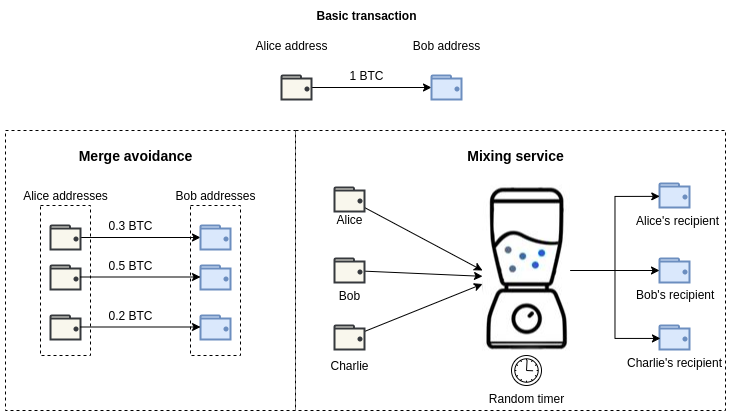
\includegraphics[width=\textwidth]{Images/mixing_merge.png}
\caption{Coin mixing and merge avoidance for transaction obfuscation.} 
\label{F_coin_mixing}
\end{figure*}

\textbf{Limitations of centralized coin mixing.} Centralized coin mixing services, although important privacy-enhancing parts in blockchains have several limitations which create significant risks for users:
\begin{itemize}
    \item \emph{availability}: being centralized and responsible for obfuscating transactions, coin mixing services are likely targets of denial-of-service attacks as single points of failure (SPOF) \cite{Sarfraz2019};
    \item \emph{trust}: the centralized mixing service needs to be trusted, as it still can link the sender and the receiver of the transaction, and also can keep the coins for itself, or take a fee without actually providing the service.
\end{itemize}

These two limitations are direct risks to the security and privacy of the users. This justifies the introduction of decentralized mixing schemes.

\textbf{Decentralized coin mixing.}
Coin mixing services, when centralized, become a single point of failure \cite{Sarfraz2019, Andola2021} and are targets of choice for attackers willing to break the privacy of users or to embezzle the coins. Therefore, the first natural step to improve coin mixing would be to decentralize the mixing service. Decentralized mixing faces a major issue nonetheless, known as the \emph{bootstrapping problem}\cite{Glaeser2022}. The bootstrapping problem is the difficulty to find a set of initial participants to execute the protocol.
While a high number of participants is desirable to improve
the anonymity guarantees provided by the coin mixing protocol, it is at the same time undesirable as it results in
poor scalability and makes bootstrapping harder \cite{Glaeser2022}. 

While decentralized mixing services are more resilient against denial of service attacks, the decentralization 
is troublesome as well as it exposes the mixing service to \emph{edge insertion attacks}.
In such attacks, a malicious user claims that additional mock nodes were involved in the mixing process to receive the corresponding rewards on their behalf \cite{Simoes2021}. While this kind of attack is easy to mitigate with a central entity accountable for node identity verification,
it becomes a challenge in a distributed setting. This attack is hard to prevent in distributed ledgers with transaction fees, as the miner, and consequently, the mixing service must be 
paid to fulfill their role and cover their costs.

\textbf{Merge avoidance.}
Merge avoidance is a technique first designed for Bitcoin \cite{Hearn2013, Simoes2021} by Mike Hearn, a Bitcoin developer, but it can be generalized to other cryptocurrencies \cite{Sarfraz2019}. In merge avoidance, a single transaction between two users is split into numerous sub-transactions for both users, hiding the amount of the original transaction. A new address must be created for each sub-transaction, and the addresses must not be linked to the identity of the sender. Otherwise, it will be easy to rebuild the original transaction using a blockchain explorer with either the sender or the receiver address.

The purpose of merge avoidance is to prevent inference attacks, in which an attacker could use the amount of cryptocurrency sent to infer the purpose of the transaction. For instance, let's consider a case where Alice is getting paid her wage in the Ethereum cryptocurrency (ETH). Each month, she gets her wage to the same wallet, at a similar time of the month. An attacker can easily guess the purpose of the transaction by observing the different transactions with Alice's wallet as outputs. By sending each individual wage in different sub-transactions to multiple wallets belonging to Alice, it is much harder to identify the purpose of the payments.
However, the merge avoidance strategy has downsides \cite{Hearn2013}:

\begin{itemize}
    \item as a receiver, your level of privacy depends on the sender and how it crafts transactions. However, the senders do not have a strong incentive to protect your privacy and may just ignore the merge avoidance process if it is not compulsory;  
    \item it increases the number of transactions, which increases the size of the ledger, but the overhead is quite limited \cite{Hearn2013};
\end{itemize}

\subsection{Privacy-oriented cryptocurrencies}

While privacy-enhancing technologies have been devised to preserve the privacy of blockchain users, other cryptocurrencies endeavor to implement privacy by design. Here are a few technologies of interest focusing on privacy protection:

\textbf{Monero} (XMR): Monero \cite{Saberhagen2013} is a privacy-focused cryptocurrency that uses a technology called \emph{ring signatures} to mask the sender's identity. It relies on stealth addresses to conceal the recipient's address and \emph{ring confidential transactions} (RingCT) to obfuscate the transaction amount. These techniques make it difficult to trace Monero transactions and provide a high level of privacy.

\textbf{Zcash} (ZEC): Zcash \cite{Bowe2016} is a privacy-oriented cryptocurrency that uses a technology called \emph{zero-knowledge proofs} (ZKPs) to keep transactions private. ZKPs allow users to prove that a statement is true without revealing any additional information beyond what is necessary \cite{Goldwasser1985}. In Zcash, ZKPs are used to hide transaction details such as the sender's address, the recipient's address, and the transaction amount.

\textbf{Dash} (DASH): Dash \cite{Duffield2014}is a privacy-focused cryptocurrency that offers optional privacy features. Dash seeks to improve upon Bitcoin (BTC) by providing stronger privacy and faster transactions. Its \emph{PrivateSend} feature allows users to mix their transactions with other users to make them more difficult to trace. PrivateSend uses a decentralized network of \emph{masternodes} to mix transactions, ensuring that no single entity can track the transaction history.

\subsection{Conclusion on privacy}
\label{ss_conclusion_on_privacy}

While blockchain transactions are often considered privacy-preserving, distributed led/- gers are confronted with challenges when protecting users' anonymity. Distributed ledgers often only provide pseudonymity, which can be broken by some actors notably by using network information. Some privacy-enhancing technologies have been designed to safeguard users' anonymity, such as the coin mixer, whose purpose is to prevent the linkage between the sender and the receiver of a transaction. Additionally, some cryptocurrencies have been designed to specifically provide anonymous transactions (ZCash, Monero...). In the next section, we will discuss the performance aspects of DLT, such as the metrics used to describe the performance of a distributed ledger, as well as the impact of the consensus methods on these metrics. 
\section{Performance considerations of distributed ledger technologies}
\label{S_DLT_performance}

Due to resource-consuming and time-consuming consensus methods, blockchains and distributed ledger performances have been critically important in the literature. \cite{Brotsis2021, Fan2021, Chen2022, Okegbile2022}. 
Performance aspects are the basis used to compare consensus methods and suggest or preclude the use of a consensus method for a use case. In this section, we will first introduce the metrics used to assess the performance of a consensus method (Section \ref{ss_performance_metrics}), before detailing the expected performance of the most important methods and how they answer the Internet of Things requirements (Section \ref{ss_performance_consensus_methods}). 

% Finally, in Section \ref{ss_suitability_iot}, the suitability of the distributed ledgers for the Internet of Things is assessed, based on their expected performance.

\subsection{Performance metrics}
\label{ss_performance_metrics}

To assess the performance of distributed ledger technologies, a wide range of parameters can be considered. Security aspects must also be considered as increasing performance may impact security negatively. In distributed ledger technologies, this translates into a relatively low adversary tolerance. \emph{Adversary tolerance} is achieved through designing consensus protocols that guarantee security even in the presence of an adversary who may control up to a certain fraction of the resources of the system. This fraction expresses the robustness of the consensus method. We now look at the different metrics used to measure the performance of a consensus method.

\textbf{Throughput}, or in the context of distributed ledger, transaction throughput, is the number of transactions that a blockchain network can process per unit of time. It is usually expressed in \emph{transaction per second} (TPS). It must be distinguished from \emph{network throughput}, which measures the amount of data that can be transmitted from one point to another within a given time. It is usually expressed in bits per second (bps) or bytes per second (Bps) but is a less relevant notion for blockchain networks. Transaction throughput can greatly vary when comparing DLTs. The Bitcoin blockchain has a maximum throughput of around 3-7 transactions per second, while Ethereum, the $2^{nd}$ most important blockchain in capitalization has a throughput between 15 and 45 TPS in its current version \footnote{Ethereum 2.0 is expected to drastically increase the throughput}. Compared with traditional payment networks, Visa can process up to 24.000 transactions per second, while Paypal has a 193 TPS throughput. A final thing to consider when discussing throughput is the range. A network processing under 100 transactions per second can be considered as having a low throughput, while 100 to 1000 TPS will be considered average and over 100 TPS a high throughput \cite{Salimitari2020}.

\textbf{Latency}, in blockchain networks, is the amount of time between initiating a transaction or payment and receiving confirmation that it is valid \cite{Kokoris-Kogias2022}. It is sometimes referred to as \emph{block time}, which covers a slightly different notion as blocks are not transactions, but groups of transactions. For instance, a block of the Bitcoin blockchain can be made of 2000 transactions \cite{nasdaq2023}. Latency is usually expressed in seconds.
While latency may seem to be the inverse of throughput, these two notions are not related. Indeed, when the system is at a low load, the number of transactions per second can increase until reaching the high load regime for the network, with no impact on the latency. Conversely, on high load, if new transactions are pushed to the network, the throughput stays the maximum, but the latency keeps on increasing. Both notions are therefore necessary to reflect the transaction processing capacity of a given distributed ledger network. 

\textbf{Scalability}, which actually covers two different concepts~\cite{Steen2020}. First, scalability in terms of transaction processing capacity, and can be considered as throughput. Then, scalability in terms of the number of users, which is positively impacted by the open membership, the lack of any centralized component and the absence of trust assumptions on any third-party~\cite{Steen2020}. Scalability is consequently strongly related to decentralization. As set in assumptions (cf. Section \ref{S_assumptions}), only large-scale IoT networks are considered in this thesis, which implies that high scalability is compulsory. Despite being crucial, it is also one of the most difficult metrics to evaluate accurately.

\textbf{Network overhead}.
In the context of distributed ledgers, network overhead refers to the amount of additional data transmitted over the network that is required to support the consensus protocol, verify transactions, or maintain the distributed ledger system. This additional data can include message headers, authentication and encryption data, transaction data, and consensus-related data, and can increase the total amount of network traffic required to operate the system. This is a metric of interest for the Internet of Things, as a high network overhead will limit the scalability in terms of nodes.

\textbf{Storage overhead} is the additional storage space required to maintain the ledger, including transaction data and metadata, on each node in the network. Internet of Things devices e.g., sensors, may have very low storage. A high storage overhead excludes low storage devices from contributing to the consensus method.
\rul{Additionally, devices must store basic knowledge of the network even though they do not contribute to the network as a node. In particular, devices need to store network configuration information to connect to the network. This includes details such as the IP addresses and ports of nodes it will communicate with.  Each IoT device should also store its private keys associated with its addresses. The private keys allow the device to sign transactions and prove ownership of the associated addresses and coins.}
\subsection{Performance of consensus methods}
\label{ss_performance_consensus_methods}

Using the above-mentioned performance metrics (cf. Section \ref{ss_performance_metrics}), we discuss how consensus methods compare with each other. In particular, we highlight which distributed ledger technologies are suitable for the Internet of Things from a performance perspective, i.e., regardless of security and privacy concerns. The discussion is summarized in Table \ref{tab:performance_dlt}.

\textbf{Proof of Work.} The PoW is a consensus method based on a computation-intensive cryptographic puzzle. The difficulty of the cryptographic challenge directly defines the security and the performance of the network. By design, PoW-based blockchains usually have a low throughput and a high latency to allow time for the nodes to check the new transactions' correctness. Storage is troublesome as well, as the size of the ledger is continuously increasing and can not be stored on a device with low capacity. PoW is consequently not adapted for the Internet of Things.

\textbf{Proof of Stake.} The proof of stake removes the computation race between nodes, alleviating computation requirements compared to the proof of work. However, throughput is still low considering IoT requirements \cite{Raghav2020}. As it is a monetary-based approach, it is often excluded for IoT use cases \cite{Raghav2020, Salimitari2020}, as it requires constrained devices to hold a cryptocurrency. The proof of stake also tends to concentrate the power into the hands of the richest nodes, centralizing the network to some extent \cite{Salimitari2020}. The \textbf{Proof of Authority} is very similar to the proof of stake but does not introduce monetary concepts.

\textbf{Delegated Proof of Stake.} Electing miners and nodes responsible for the network management significantly improves throughput and latency, but centralizes the network. Besides, it also requires holding a cryptocurrency to participate in the voting, limiting its adoption in the Internet of Things.

\textbf{Proof of Elapsed Time.} The proof of elapsed time has a low latency and a high throughput and can be considered IoT-friendly \cite{Salimitari2020}. The only drawback is the need to verify the timer's execution using a dedicated \emph{Trusted Execution Environment}. For PoET, it is usually done using Intel's SGX software, which makes it partly centralized and limits its use in large-scale networks.

\textbf{Practical Byzantine Fault Tolerance.} Similarly to PoET, PBFT features high throughput, low latency and low computational overhead making it appealing for IoT networks. However, PBFT requires a lot of messages to achieve consensus and has a high network overhead, strongly limiting its scalability and restricting its use to private blockchains and small IoT networks. The \textbf{delegated Byzantine Fault Tolerance} does not require the participation of all nodes in the consensus, aiming at solving the network overhead issue, but at the cost of higher latency making it unsuitable for the Internet of Things \cite{Salimitari2020}.

\textbf{IOTA.} IOTA has been specifically designed for the Internet of Things requirements. IOTA provides high throughput and low latency for transactions, as well as high scalability \cite{Alshaikhli2022}. Nodes do not require to store the whole ledger to run, rather relying on automated snapshotting, limiting storage overhead. \rul{IOTA is introduced in detail in Chapter} \ref{C_solving_trilemma} (Section \ref{S_iota_dlt})\rul{ and is identified as a crucial technology for the Internet of Things.}
\begin{table*}
\begin{center}
 \begin{scriptsize}
\setlength{\extrarowheight}{12pt}
\begin{adjustbox}{angle=90}
\begin{tabular}{ |c|c|c|c|c|c|c|c|c|} 
\hline
Consensus method & Scalability & Latency & Throughput & Adversary tolerance & Network overhead & Storage overhead & IoT suitable\\
\hline
PoW & High & High & Low  & <51\% computing power & Low & High & \xmark \\ 

PoS & High & Medium & Low & <51\% stakes & Low & High & ?\\ 

PoA & High & Medium & Low & <51\% stakes & Low & High & ?\\

DPoS & High & Medium & High & <51\% validators & n/a & High & ?\\

PoET & High & Low & High & n/a & Low & High & \cmark (small scale)\\

PBFT & Low & Low & High & <33\% faulty replicas & High & High & \cmark (small scale)\\ 

dBFT & High & Medium & High & <33\% faulty replicas & High & High & \xmark\\ 

IOTA & High & Low & High & <33\% computing power & Low & Low & \cmark\\ 

\hline

\end{tabular}
\end{adjustbox}
\captionof{table}{Performance of consensus methods - based on \cite{Salimitari2020}}
\label{tab:performance_dlt}
 \end{scriptsize}
\end{center}
\end{table*}


\section{Conclusion}
\label{S_conclusion_state_of_the_art}
In this chapter, we introduced the state of the art on usage control and on distributed ledger technologies needed to understand the context and the contributions of this 
thesis. First, we highlighted the purpose of usage control and information flow control to monitor data usage and data dissemination (Section \ref{S_usage_control}). Then, distributed ledger 
technologies have been extensively discussed, from general considerations (Section \ref{ss_DLT_elementaries}) to privacy challenges (Section \ref{S_privacy_DLT}). Finally,
we addressed performance aspects of distributed ledgers, which are paramount considering Internet of Things constraints. The performance of 
a distributed ledger technology is deeply correlated to the method used to achieve consensus.

In the following chapters, the different contributions of this thesis are described. The next chapter \ref{C_solving_trilemma} introduces a framework for efficient, privacy-preserving zero-fee transactions in the Internet of Things (\hyperref[obj:1]{\emph{Objective 1}}).
The framework is based on the aforementioned technologies, notably usage control, distributed ledgers and privacy-enhancing technologies 
for transactions, motivating this chapter on the state of the art and its analysis.
